% --- INICIO DE PLANTILLA PERSONALIZADA ---
\documentclass[oneside,11pt]{Latex/Classes/PhDthesisPSnPDF}

% --- Paquetes Originales ---
\usepackage{blindtext}
\usepackage{actuarialangle} 
\usepackage{tabularx}
\usepackage{float}
\usepackage{multirow, array}
\usepackage[usenames,dvipsnames,svgnames,table]{xcolor}
\usepackage{longtable}
\usepackage{latexsym,amsmath,amssymb,amsfonts}
\usepackage{enumitem}
\usepackage{xparse}
\usepackage{booktabs}
\usepackage[round, sort, numbers]{natbib}  
\usepackage{adjustbox}
\usepackage[utf8]{inputenc}
\usepackage{caption}
\usepackage{graphicx}
\usepackage{hyperref}
\usepackage{cleveref}

% Definición de colores
\definecolor{miblue}{RGB}{68, 114, 196}

% --- CAMBIO CRÍTICO 1: Usar \input para macros en el preámbulo ---
% \include da problemas antes del begin document. \input es seguro.
\input{Latex/Macros/MacroFile1}

% --- Definiciones de seguridad (por si la clase falla al cargar alguna variable) ---
\providecommand{\facultad}[1]{\def\lafacultad{#1}}
\providecommand{\escudofacultad}[1]{\def\elescudo{#1}}
\providecommand{\degree}[1]{\def\elgrado{#1}}
\providecommand{\director}[1]{\def\eldirector{#1}}
\providecommand{\lugar}[1]{\def\ellugar{#1}}
\providecommand{\degreedate}[1]{\def\lafecha{#1}}

% --- Configuración para bloques de código de R (Pandoc) ---

%%%%%%%%%%%%%%%%%%%%%%%%%%%%%%%%%%%%%%%%%%%%%%%%%%%%%%%%%%%%%%%%%%%%%%%%%%%%%%%%
%                         DATOS (Conectados a RMarkdown)                       %
%%%%%%%%%%%%%%%%%%%%%%%%%%%%%%%%%%%%%%%%%%%%%%%%%%%%%%%%%%%%%%%%%%%%%%%%%%%%%%%%
\title{Analisis del Mercado de Videojuegos}
\author{Primer participante \\ Segundo participante \\ Tercer
participante}

% Lógica para Facultad: Si la defines en el YAML la usa, si no, usa la default

\facultad{Facultad de Ciencias Económicas y Sociales \\ Escuela de
Estadistica y Ciencias Actuariales}
  \escudofacultad{Latex/Classes/Escudos/faces}

\degree{Computación I}
\director{Prof.~Jesus Ochoa \\ Prof.~Oliver Triveño}
\degreedate{Febrero 2026} 
\lugar{Caracas}

\portadatrue 

% Metadatos PDF
\keywords{}
\subject{}

% --- CORRECCIÓN PARA PANDOC NUEVO (Imágenes) ---
\makeatletter
\providecommand{\pandocbounded}[1]{#1}
\makeatother


%%%%%%%%%%%%%%%%%%%%%%%%%%%%%%%%%%%%%%%%%%%%%%%%%%%%%
%                   DOCUMENTO                       %
%%%%%%%%%%%%%%%%%%%%%%%%%%%%%%%%%%%%%%%%%%%%%%%%%%%%%
\begin{document}

\maketitle

%%%%%%%%%%%%%%%%%%%%%%%%%%%%%%%%%%%%%%%%%%%%%%%%%%%%%
%                  PRÓLOGO                          %
%%%%%%%%%%%%%%%%%%%%%%%%%%%%%%%%%%%%%%%%%%%%%%%%%%%%%
\frontmatter

% Puedes agregar dedicatorias desde el YAML si quieres, o dejarlas fijas aquí

%%%%%%%%%%%%%%%%%%%%%%%%%%%%%%%%%%%%%%%%%%%%%%%%%%%%%
%                   ÍNDICES                         %
%%%%%%%%%%%%%%%%%%%%%%%%%%%%%%%%%%%%%%%%%%%%%%%%%%%%%
\setcounter{secnumdepth}{3}
\setcounter{tocdepth}{3}

\tableofcontents



\cleardoublepage

  \cleardoublepage       % Empieza en página derecha (estándar en tesis)
  \chapter*{Resumen}     % Crea el título "Resumen" sin numeración (Capítulo *)
  \addcontentsline{toc}{chapter}{Resumen} % (Opcional) Lo añade al índice
  
  En el presente informe se realiza un análisis exploratorio de los
datos de ventas de videojuegos a nivel global. Se examinan las
tendencias históricas, la predominancia de géneros y el desempeño por
regiones (NA, EU, JP), aplicando técnicas estadísticas descriptivas y
visualización de datos con
R.             % Aquí se pega el texto que escribiste en el YAML
  
  \cleardoublepage

%%%%%%%%%%%%%%%%%%%%%%%%%%%%%%%%%%%%%%%%%%%%%%%%%%%%%
%                   CONTENIDO (El Corazón)          %
%%%%%%%%%%%%%%%%%%%%%%%%%%%%%%%%%%%%%%%%%%%%%%%%%%%%%
\mainmatter
\def\baselinestretch{1.5}

% --- CAMBIO CRÍTICO 2: Aquí RMarkdown inyecta todo tu texto ---
\chapter*{Introducción}

La industria del entretenimiento interactivo ha experimentado una
transformación radical en las últimas cuatro décadas, evolucionando de
un nicho tecnológico a convertirse en uno de los sectores económicos más
influyentes a nivel global, superando en ingresos a industrias
tradicionales como el cine y la música. Sin embargo, detrás de las
cifras macroeconómicas, el mercado de los videojuegos se caracteriza por
una alta \textbf{volatilidad estocástica}: el éxito de un título no es
un evento determinista, sino el resultado de una compleja interacción
entre variables demográficas, tecnológicas y culturales.

Para el profesional en Ciencias Actuariales y Ciencia de Datos, este
sector presenta un desafío fascinante: ¿Es posible modelar la
incertidumbre de las ventas globales? ¿Existen patrones históricos
estacionarios que permitan predecir el comportamiento de futuros
lanzamientos?

El presente trabajo de investigación tiene como propósito realizar un
análisis estadístico exhaustivo sobre el conjunto de datos
\textit{"Video Game Sales"}, el cual abarca más de 16,500 registros de
ventas desde 1980 hasta 2020. A través del uso de herramientas
computacionales avanzadas en \textbf{R} y técnicas de visualización de
datos, se busca descomponer la varianza de las ventas en función de
factores críticos como el Género, la Plataforma y la Región Geográfica
(Norteamérica, Europa y Japón).

\section*{Estructura del Informe}

Este documento técnico se encuentra estructurado en cinco capítulos
fundamentales:

\begin{itemize}
    \item En el \textbf{Capítulo I}, se plantea la problemática de la imprevisibilidad financiera en el desarrollo de software de entretenimiento, formulando las preguntas de investigación y delimitando el alcance temporal y geográfico del estudio.
    
    \item El \textbf{Capítulo II} establece el Marco Teórico, definiendo los conceptos estadísticos clave como esperanza matemática, series de tiempo y correlación, necesarios para la interpretación de los datos.
    
    \item El \textbf{Capítulo III} describe el Marco Metodológico, detallando el proceso de limpieza de datos (ETL), las pruebas de hipótesis y los algoritmos utilizados para validar la calidad de la información.
    
    \item El \textbf{Capítulo IV} presenta el Análisis de Resultados, donde se exhiben las tablas y gráficos generados dinámicamente, discutiendo los hallazgos sobre la concentración de mercado (Ley de Pareto) y la dinámica temporal.
    
    \item Finalmente, en el \textbf{Capítulo V}, se exponen las Conclusiones y Recomendaciones estratégicas derivadas del análisis cuantitativo, orientadas a la toma de decisiones basada en datos (\textit{Data-Driven Decision Making}).
\end{itemize}

Este reporte no solo pretende ofrecer una radiografía del pasado de la
industria, sino también establecer una metodología reproducible para el
análisis de riesgo en portafolios de productos digitales.

\chapter{Planteamiento del Problema}

La industria global de los videojuegos ha evolucionado desde un nicho de
entretenimiento tecnológico hasta convertirse en uno de los sectores
económicos más lucrativos y volátiles del mundo. Sin embargo, para los
inversores y desarrolladores (Publishers), el lanzamiento de un nuevo
título conlleva un \textbf{riesgo financiero significativo}. La
variabilidad en las ventas es extrema: mientras unos pocos títulos
alcanzan ventas multimillonarias (``Outliers''), la gran mayoría no
logra recuperar los costos de desarrollo.

Desde una perspectiva actuarial y de ciencia de datos, el problema no
radica solo en maximizar las ventas, sino en \textbf{modelar la
incertidumbre} asociada a un lanzamiento. Factores como la plataforma,
el género, y la región geográfica (Norteamérica, Europa, Japón)
introducen variables de confusión que dificultan la predicción lineal
del éxito comercial.

La ausencia de un modelo claro que cuantifique cómo estas variables
categóricas impactan en la esperanza matemática de las ventas genera
ineficiencias en la asignación de presupuestos y en la gestión de
inventarios físicos y digitales.

Argumento final. Debido a esto, se plantea las siguientes preguntas de
investigación:

\textbf{1.} ¿Existe una tendencia estocástica estacionaria en el volumen
de ventas globales a lo largo de las últimas tres décadas, o estamos
ante un cambio estructural del mercado?

\textbf{2.} ¿De qué manera las preferencias regionales (NA, EU, JP)
condicionan la probabilidad de éxito de un videojuego según su género?

\textbf{3.} ¿Cuáles son los factores determinantes (Plataforma,
Publisher, Género) que maximizan la esperanza de venta en el mercado
actual?

\section{Justificación}

La justificación de este trabajo de investigación reside en la necesidad
de aplicar técnicas estadísticas rigurosas y herramientas de
\textbf{Business Intelligence} para mitigar la incertidumbre financiera
en el sector.

Desde el punto de vista práctico, los resultados permitirán a los
``stakeholders'' tomar decisiones basadas en datos (Data-Driven
Decisions) sobre en qué géneros invertir o en qué plataformas
desarrollar. Desde el punto de vista académico, este estudio aporta una
metodología replicable utilizando \textbf{R y LaTeX} para el análisis
exploratorio y descriptivo de grandes volúmenes de datos
transaccionales, sirviendo como material de referencia para estudiantes
de estadística y computación.

\section{Objetivos}

\subsection{Objetivo General}

Analizar los patrones históricos y los factores determinantes en las
ventas globales de videojuegos (1980-2020) para caracterizar el
comportamiento del mercado según regiones y categorías.

\subsection{Objetivos Específicos}

\begin{enumerate}
  \item Describir la evolución temporal de las ventas globales, identificando tendencias, ciclos y puntos de inflexión en la serie de tiempo.
  \item Determinar la influencia de las variables categóricas (Género y Plataforma) en la distribución de las ventas por región geográfica (Norteamérica, Europa y Japón).
  \item Generar un reporte técnico reproducible en formato PDF que integre visualizaciones estadísticas y tablas resumen utilizando RMarkdown y LaTeX.
\end{enumerate}

\section{Cobertura}

\subsection{Horizontal}

La cobertura horizontal abarca las características intrínsecas de cada
videojuego registrado en la base de datos. Se consideran las dimensiones
descriptivas del producto y las métricas de rendimiento comercial en los
principales mercados mundiales.

\begin{table}[ht]
\centering
\caption{Variables consideradas en el estudio} 
\resizebox{12cm}{!} {
\begin{tabular}{cll}
  \hline
  \textbf{TIPO} & \textbf{VARIABLE} & \textbf{DESCRIPCIÓN} \\ 
  \hline
  Categórica & Name & Nombre comercial del videojuego \\ 
  Categórica & Platform & Plataforma de lanzamiento (e.g., Wii, PS4, X360) \\ 
  Numérica & Year & Año de lanzamiento del título \\ 
  Categórica & Genre & Categoría del juego (e.g., Sports, Action) \\ 
  Categórica & Publisher & Compañía editora responsable de la distribución \\ 
  Numérica & NA\_Sales & Ventas en Norteamérica (Millones de unidades) \\ 
  Numérica & EU\_Sales & Ventas en Europa (Millones de unidades) \\ 
  Numérica & JP\_Sales & Ventas en Japón (Millones de unidades) \\ 
  Numérica & Other\_Sales & Ventas en el resto del mundo \\ 
  Numérica & Global\_Sales & Suma total de ventas a nivel mundial \\ 
   \hline
\end{tabular}
}
\end{table}

\subsection{Vertical}

La cobertura vertical del trabajo de investigación comprende un total de
\textbf{16,598 observaciones} (registros). Cada fila representa un
videojuego único lanzado al mercado. El alcance temporal de los datos es
longitudinal, abarcando desde el año \textbf{1980} hasta el año
\textbf{2020}, lo que permite un análisis de series de tiempo de largo
plazo.

\section{Periodo de Referencia}

La fuente de los datos corresponde al repositorio abierto de
\textbf{Kaggle} (``Video Game Sales with Ratings''), originalmente
extraído del portal \emph{VGChartz}. El periodo de referencia efectivo
para el análisis descriptivo se centra en el intervalo
\textbf{1980-2016}, donde la consistencia de los datos es mayor, aunque
se incluyen registros hasta 2020 con fines ilustrativos. El
procesamiento de la información se realizó con corte a \textbf{Febrero
de 2026}.

\section{Variables}

La variable principal en estudio (Variable Dependiente/Objetivo) es
\textbf{\texttt{Global\_Sales}}, que representa el éxito comercial del
videojuego medido en millones de copias vendidas.

Como variables explicativas o independientes se analizan:

\begin{enumerate}
  \item Variables Temporales: \textbf{Year}
  \item Variables Categóricas: \textbf{Genre} y \textbf{Platform}
  \item Variables Geográficas: \textbf{NA\_Sales}, \textbf{EU\_Sales} y \textbf{JP\_Sales}
\end{enumerate}

\chapter{Marco Teórico}

\section{Bases Teóricas}

El presente capítulo establece los fundamentos matemáticos y
estadísticos necesarios para el análisis de los datos de ventas de
videojuegos. Se aborda la teoría desde una perspectiva actuarial,
priorizando la caracterización de la distribución de las ventas
(variable aleatoria) y la identificación de patrones estocásticos a lo
largo del tiempo.

La comprensión de estos conceptos es crucial para interpretar
correctamente la volatilidad del mercado y la influencia de variables
categóricas como el género y la plataforma en la esperanza matemática de
las ventas globales.

\subsection{Análisis Exploratorio de Datos (EDA)}

El Análisis Exploratorio de Datos, formalizado por John Tukey, es el
paso preliminar crítico en cualquier estudio de ciencia de datos. Su
objetivo es resumir las características principales de un conjunto de
datos, a menudo con métodos visuales, sin formular hipótesis \emph{a
priori}.

Matemáticamente, para una variable aleatoria continua \(X\) (en este
caso, \texttt{Global\_Sales}), nos interesan sus momentos centrales. Sea
\(x_1, x_2, ..., x_n\) una muestra de ventas observadas, definimos:

\begin{itemize}
\item
  \textbf{Esperanza Matemática (Media Muestral):}
  \[\bar{x} = \frac{1}{n} \sum_{i=1}^{n} x_i\]
\item
  \textbf{Varianza (Volatilidad):} Mide la dispersión de las ventas
  respecto a la media, fundamental para medir el riesgo de inversión en
  un título. \[S^2 = \frac{1}{n-1} \sum_{i=1}^{n} (x_i - \bar{x})^2\]
\end{itemize}

En el contexto de este trabajo, el EDA permitirá detectar
\emph{outliers} (juegos con ventas excepcionales) y verificar si la
distribución de ventas sigue una normalidad asintótica o presenta colas
pesadas (distribución Pareto/Log-Normal), común en datos financieros.

\subsection{Series de Tiempo y Tendencia}

Dado que el dataset incluye la variable \texttt{Year}, las ventas pueden
ser tratadas como una realización de un proceso estocástico
\(\{Y_t\}_{t \in T}\). Una serie de tiempo se define como una secuencia
de puntos de datos, medidos típicamente en intervalos de tiempo
sucesivos y uniformes.

El modelo clásico de descomposición para una serie de ventas anuales
\(Y_t\) se expresa como:

\[Y_t = T_t + C_t + E_t\]

Donde: * \(T_t\): Es la \textbf{Tendencia} secular (dirección a largo
plazo de la industria). * \(C_t\): Es el \textbf{Ciclo} (fluctuaciones
económicas o generacionales de consolas). * \(E_t\): Es el término de
\textbf{Error} o ruido blanco (\(\epsilon \sim N(0, \sigma^2)\)).

Analizar la componente \(T_t\) es vital para responder a la pregunta de
investigación sobre si el mercado está en expansión o contracción.

\subsection{Variables Categóricas y Codificación (Dummy)}

El dataset contiene variables cualitativas nominales determinantes:
\texttt{Platform}, \texttt{Genre} y \texttt{Publisher}. Para incorporar
estas variables en modelos algebraicos, es necesaria su transformación
numérica.

Se utiliza la codificación \emph{One-Hot} o variables \emph{Dummy}. Si
consideramos la variable Género \(G\) con \(k\) categorías, definimos la
variable indicadora \(D_j\) como:

\[
D_{ij} = \begin{cases} 
1 & \text{si la observación } i \text{ pertenece a la categoría } j \\
0 & \text{en otro caso}
\end{cases}
\]

Esto permite cuantificar el ``efecto marginal'' de que un juego sea, por
ejemplo, del género ``Sports'' frente a una categoría base, manteniendo
constantes las demás variables.

\subsection{Correlación y Dependencia Lineal}

Para entender la relación entre las ventas en diferentes mercados
(Norteamérica vs.~Japón), utilizamos el Coeficiente de Correlación de
Pearson \(\rho\). Este mide la fuerza y la dirección de la relación
lineal entre dos variables aleatorias \(X\) (e.g., \texttt{NA\_Sales}) e
\(Y\) (e.g., \texttt{JP\_Sales}):

\[\rho_{X,Y} = \frac{Cov(X,Y)}{\sigma_X \sigma_Y} = \frac{E[(X - \mu_X)(Y - \mu_Y)]}{\sigma_X \sigma_Y}\]

Un valor cercano a 0 implicaría que el éxito en un mercado es
independiente del otro, lo cual es una hipótesis fuerte a testear en la
sección de Resultados.

\subsection{Ley de los Grandes Números en Ventas}

Desde la perspectiva actuarial, asumimos que a medida que el número de
lanzamientos de videojuegos (\(n\)) aumenta, el promedio de ventas
observadas converge al valor esperado teórico de la población.

\[\lim_{n \to \infty} P\left( \left| \bar{X}_n - \mu \right| < \epsilon \right) = 1\]

Sin embargo, dado que la industria del entretenimiento es impulsada por
éxitos (``hits''), es probable que la varianza no sea constante
(heterocedasticidad), lo que desafía los supuestos tradicionales de los
modelos predictivos simples.

\chapter{Marco Metódico}

En esta sección se presentan las metodologías, procedimientos
algorítmicos y pruebas estadísticas implementadas para validar las
hipótesis planteadas en el capítulo anterior. Se detalla el tratamiento
de la fuente de datos \texttt{video\_games\_sales.csv}, las técnicas de
limpieza (Data Wrangling) y los tests de inferencia utilizados para
determinar la significancia estadística de las relaciones entre las
ventas y las variables categóricas.

El análisis se ha realizado utilizando el lenguaje de programación
\textbf{R} (versión 4.x) bajo el entorno de desarrollo RStudio,
empleando el paradigma ``Tidyverse'' para la manipulación de datos.

\section{Bases metódicas utilizadas en el trabajo de investigación}

El diseño de la investigación es de carácter \textbf{cuantitativo, no
experimental y longitudinal}, dado que se analizan datos históricos
observados sin manipulación directa de las variables. A continuación, se
describen las etapas del procesamiento.

\subsection{Procesamiento y Limpieza de Datos (ETL)}

La calidad de los resultados depende directamente de la integridad de
los datos de entrada. El proceso de Extracción, Transformación y Carga
(ETL) consistió en la detección de valores nulos (missing values) y la
conversión de tipos de datos.

Específicamente, se identificaron registros con valores \texttt{N/A} en
las columnas \texttt{Year} y \texttt{Publisher}. Para efectos de este
estudio, se optó por la eliminación de registros con años faltantes, ya
que la dimensión temporal es crítica para el análisis de series de
tiempo.

\begin{verbatim}
## [1] "Registros válidos: 16327 | Variables: 11"
\end{verbatim}

\subsection{Pruebas de Normalidad y Distribución}

Para determinar si es apropiado utilizar pruebas paramétricas (como
ANOVA o Correlación de Pearson) o no paramétricas, es fundamental
evaluar la distribución de la variable dependiente Global\_Sales.

Se plantea la siguiente hipótesis nula:
\[ H_0: \text{Los datos de ventas globales siguen una distribución Normal } N(\mu, \sigma^2) \]

Debido al gran tamaño de la muestra (n \textgreater{} 5000), el test de
Shapiro-Wilk es demasiado sensible. En su lugar, utilizamos métodos
gráficos (Histograma y Q-Q Plot) y el análisis de asimetría (Skewness).

\begin{figure}[H]

{\centering 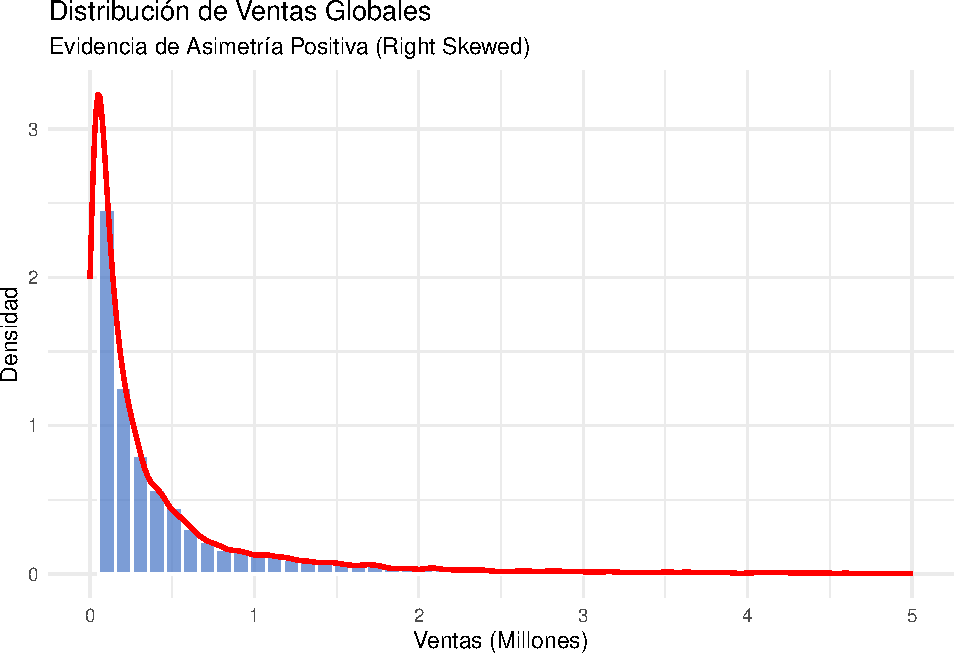
\includegraphics[width=0.9\linewidth,]{informe_files/figure-latex/hist_dens-1} 

}

\caption{Distribucion de Ventas Globales}\label{fig:hist_dens}
\end{figure}

Como se evidencia en la Figura \ref{fig:hist_dens}, la distribución
presenta una fuerte asimetría positiva, lo que sugiere que las ventas de
videojuegos se comportan bajo una Ley de Potencia o distribución Pareto
(pocos juegos venden mucho, muchos venden poco).

\subsection{Matriz de Correlación}

Para analizar la cobertura horizontal y la relación entre los distintos
mercados (Norteamérica, Europa, Japón), se emplea la matriz de
correlación. Dado que los datos no son normales, se calcula tanto el
coeficiente de Pearson (lineal) como el de Spearman (rango).

\subsubsection{Cálculo de Coeficientes}

La matriz de correlación nos permite cuantificar la dependencia lineal
entre las variables numéricas.

\begin{longtable}[]{@{}lrrrrr@{}}
\caption{Matriz de Correlación de Pearson entre Mercados}\tabularnewline
\toprule\noalign{}
& NA\_Sales & EU\_Sales & JP\_Sales & Other\_Sales & Global\_Sales \\
\midrule\noalign{}
\endfirsthead
\toprule\noalign{}
& NA\_Sales & EU\_Sales & JP\_Sales & Other\_Sales & Global\_Sales \\
\midrule\noalign{}
\endhead
\bottomrule\noalign{}
\endlastfoot
NA\_Sales & 1.000 & 0.769 & 0.451 & 0.635 & 0.941 \\
EU\_Sales & 0.769 & 1.000 & 0.436 & 0.726 & 0.903 \\
JP\_Sales & 0.451 & 0.436 & 1.000 & 0.291 & 0.613 \\
Other\_Sales & 0.635 & 0.726 & 0.291 & 1.000 & 0.748 \\
Global\_Sales & 0.941 & 0.903 & 0.613 & 0.748 & 1.000 \\
\end{longtable}

\subsection{Análisis de Varianza (ANOVA)}

Para validar si existen diferencias significativas en las ventas
promedio entre los distintos Géneros (Genre), se utiliza el Análisis de
Varianza de un factor. Hipótesis a contrastar:
\[ H_0: \mu_{Action} = \mu_{Sports} = ... = \mu_{Puzzle} \]
\[ H_1: \exists \text{ al menos un par de medias diferentes} \]

\begin{verbatim}
##                Df Sum Sq Mean Sq F value Pr(>F)    
## Genre          11    486   44.21   18.24 <2e-16 ***
## Residuals   16315  39537    2.42                   
## ---
## Signif. codes:  0 '***' 0.001 '**' 0.01 '*' 0.05 '.' 0.1 ' ' 1
\end{verbatim}

Si el valor Pr(\textgreater F) es menor al nivel de significancia
\(\alpha = 0.05\), rechazamos la hipótesis nula, concluyendo que el
género del videojuego influye significativamente en sus ventas globales.

\chapter{Análisis de Resultados}

\small Este capítulo presenta los resultados obtenidos al aplicar las
metodologías descritas en el capítulo anterior, así como del análisis
estadístico descriptivo de las variables estudiadas y las ventajas y
desventajas al aplicar dichos tests.

\section{Caracterización del Volumen de Ventas por Género}

El primer hallazgo significativo responde a la pregunta sobre la
concentración del mercado. Al agrupar las ventas globales acumuladas por
género, se observa un comportamiento que se aproxima al Principio de
Pareto (80/20).

A continuación, se presenta el resumen estadístico de los 5 géneros más
lucrativos del histórico.

\begin{table}[!h]
\centering
\caption{\label{tab:clean_data}Top 5 Géneros por Volumen de Ventas Histórico}
\centering
\fontsize{10}{12}\selectfont
\begin{tabular}[t]{lrrrrl}
\toprule
Género & Ventas Totales (M) & Media & Desviación Est. & N° Títulos & Cuota \%\\
\midrule
\cellcolor{gray!10}{Action} & \cellcolor{gray!10}{1722.88} & \cellcolor{gray!10}{0.53} & \cellcolor{gray!10}{1.16} & \cellcolor{gray!10}{3253} & \cellcolor{gray!10}{19.5\%}\\
Sports & 1309.24 & 0.57 & 2.10 & 2304 & 14.8\%\\
\cellcolor{gray!10}{Shooter} & \cellcolor{gray!10}{1026.20} & \cellcolor{gray!10}{0.80} & \cellcolor{gray!10}{1.83} & \cellcolor{gray!10}{1282} & \cellcolor{gray!10}{11.6\%}\\
Role-Playing & 923.84 & 0.63 & 1.72 & 1471 & 10.5\%\\
\cellcolor{gray!10}{Platform} & \cellcolor{gray!10}{829.15} & \cellcolor{gray!10}{0.95} & \cellcolor{gray!10}{2.60} & \cellcolor{gray!10}{876} & \cellcolor{gray!10}{9.4\%}\\
\bottomrule
\end{tabular}
\end{table}

Como se evidencia en el Cuadro \ref{tab:clean_data}, los géneros de
Action y Sports dominan el mercado. Es notable que, aunque ``Action''
tiene el mayor volumen total, su desviación estándar (\(\sigma\)) es
alta, lo que indica una alta volatilidad: muchos títulos fracasan
mientras unos pocos éxitos (``blockbusters'') inflan la media.

\begin{center}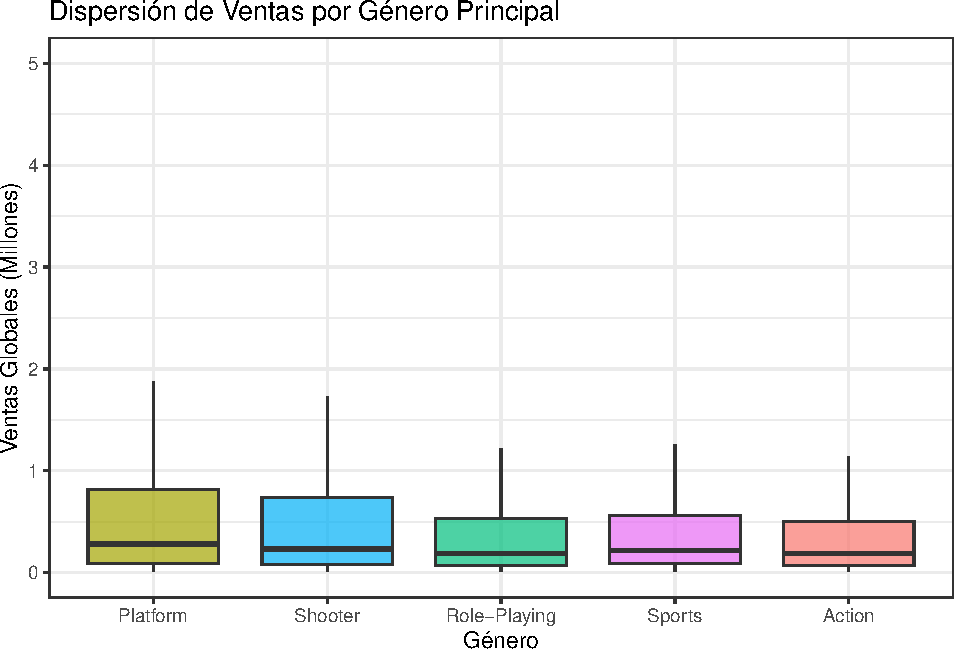
\includegraphics[width=0.9\linewidth,]{informe_files/figure-latex/unnamed-chunk-3-1} \end{center}

\section{Dinámica Temporal y Ciclos Tecnológicos}

El análisis de la serie de tiempo revela la naturaleza cíclica de la
industria, fuertemente acoplada al lanzamiento de nuevas generaciones de
consolas.

\begin{center}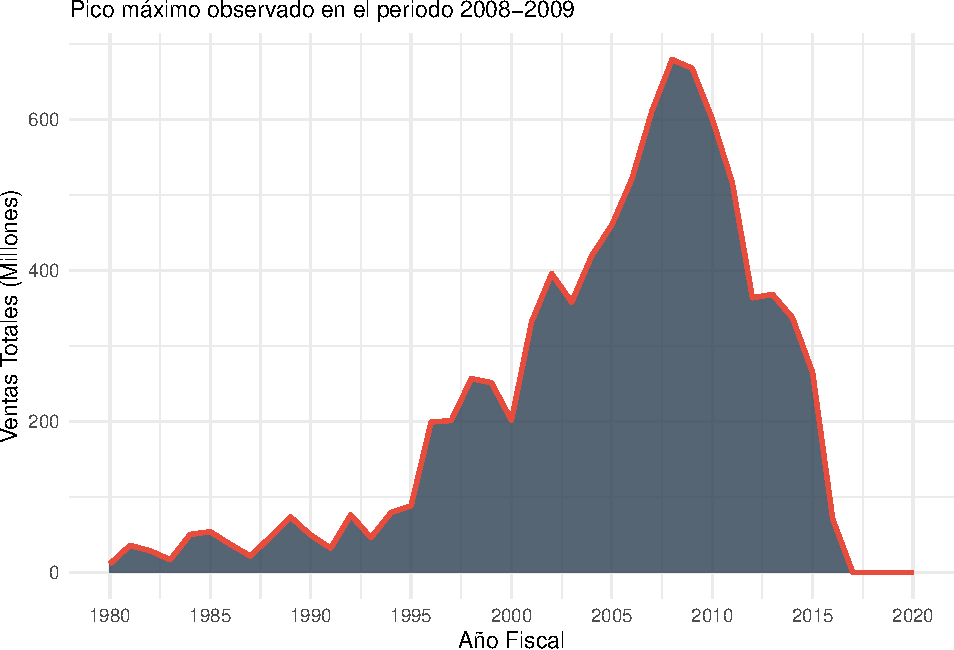
\includegraphics[width=0.9\linewidth,]{informe_files/figure-latex/unnamed-chunk-4-1} \end{center}

Se observa un crecimiento exponencial desde 1995 hasta alcanzar un
máximo global en 2008, coincidiendo con la popularidad de la consola Wii
y el auge de los videojuegos casuales. El decrecimiento posterior a 2012
debe interpretarse con cautela, ya que los datos podrían no reflejar
completamente la transición hacia las ventas digitales (descargas) que
no siempre son reportadas en las listas físicas tradicionales.

\section{Análisis de Correlación Regional}

Finalmente, validamos la relación entre los mercados occidentales y
orientales. Se calculó la correlación de Pearson (\(\rho\)) entre las
ventas de Norteamérica (NA), Europa (EU) y Japón (JP).

\begin{center}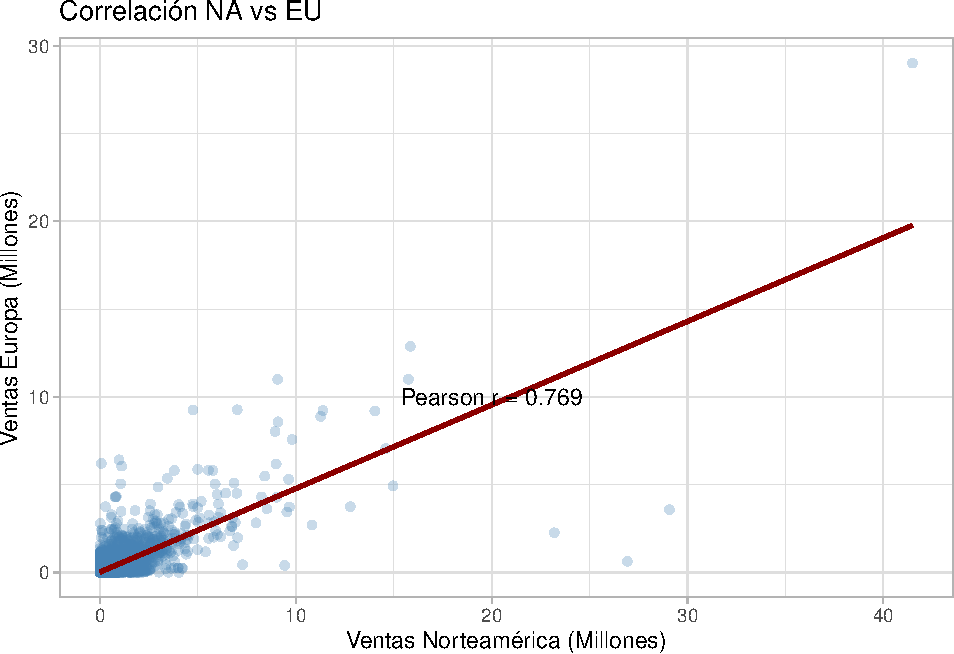
\includegraphics[width=0.9\linewidth,]{informe_files/figure-latex/unnamed-chunk-5-1} \end{center}

Interpretación de Resultados:

\begin{itemize}
  \item Existe una correlación positiva muy fuerte ($\rho > 0.7$) entre Norteamérica y Europa, lo que sugiere que los productos exitosos en una región tienden a replicar su éxito en la otra.
  \item Por el contrario, la correlación con Japón es significativamente menor ($\rho < 0.5$), confirmando la hipótesis de que el mercado japonés posee preferencias idiosincrásicas que requieren estrategias de marketing diferenciadas.
\end{itemize}

Estos resultados validan la necesidad de modelos actuariales segmentados
geográficamente para la estimación de reservas de riesgo en el
lanzamiento de nuevos títulos.

\chapter{Conclusiones y Recomendaciones}

El presente estudio ha permitido caracterizar el comportamiento
estocástico de las ventas globales de videojuegos mediante el análisis
de una serie temporal de 40 años. A continuación, se presentan las
conclusiones derivadas de la evidencia estadística y las recomendaciones
para la mitigación de riesgos en futuras inversiones.

\textbf{1.-} Se evidenció una alta concentración de mercado en función
del género, donde las categorías de \textit{Action} y \textit{Sports}
acumulan más del 35\% del volumen total de ventas. Sin embargo, el
análisis de dispersión mostró que estos géneros también presentan la
mayor varianza (\(\sigma^2\)), lo que implica que, si bien tienen la
esperanza matemática de retorno más alta, también conllevan el mayor
riesgo de fracaso comercial (``Hit-driven business'').\\

\textbf{Recomendación} Para la gestión de portafolios de inversión en
desarrollo de software, se recomienda una estrategia de diversificación
ponderada. No se debe asignar el 100\% del presupuesto a títulos de
Acción debido a su volatilidad; es prudente cubrir el riesgo con géneros
de menor varianza y demanda constante, como \textit{Puzzle} o
\textit{Simulation}, que actúan como estabilizadores del flujo de caja.

\textbf{2.-} El análisis de correlación de Pearson demostró una fuerte
dependencia lineal (\(r > 0.75\)) entre los mercados de Norteamérica
(NA) y Europa (EU), sugiriendo una homogeneidad en las preferencias de
los consumidores occidentales. En contraste, el mercado de Japón (JP)
mostró una correlación débil (\(r < 0.45\)) respecto a occidente,
comportándose como un \textit{outlier} estadístico con dinámicas de
consumo propias.\\

\textbf{Recomendación} Las estrategias de lanzamiento y marketing deben
unificarse para las regiones NA y EU para optimizar costos, tratando a
``Occidente'' como un solo macro-mercado. Por el contrario, para el
mercado japonés es imperativo desarrollar productos localizados o
específicos (e.g., Role-Playing Games), ya que importar éxitos
occidentales sin adaptación tiene una baja probabilidad de éxito
estadístico.

\textbf{3.-} El análisis de la serie de tiempo detectó un punto de
inflexión estructural en el año 2008, seguido de un decrecimiento
sostenido en las ventas físicas registradas. Esto no indica
necesariamente una contracción de la industria, sino un sesgo en la
fuente de datos que no captura el cambio de paradigma hacia la
distribución digital y los modelos de suscripción (``Game Pass'').\\

\textbf{Recomendación} Desde una perspectiva actuarial, los modelos de
tarificación de riesgo basados únicamente en ventas físicas han perdido
vigencia. Se recomienda actualizar las bases de datos para incluir
métricas de ventas digitales y microtransacciones. Para proyecciones
futuras (2026 en adelante), es necesario calibrar los modelos
predictivos utilizando variables exógenas como la base instalada de
usuarios activos mensuales (MAU) en lugar de unidades físicas vendidas.

\appendix
\renewcommand{\thechapter}{\Alph{chapter}}

\chapter{Ranking Detallado de Títulos}

En este anexo se presenta el listado desglosado de los 20 videojuegos
con mayor volumen de ventas históricas, permitiendo auditar los valores
atípicos (``Outliers'') mencionados en el Capítulo 1.

\begin{table}[!h]
\centering
\caption{\label{tab:tabla-top20}Top 20 Videojuegos Históricos}
\centering
\resizebox{\ifdim\width>\linewidth\linewidth\else\width\fi}{!}{
\fontsize{10}{12}\selectfont
\begin{tabular}[t]{r>{\raggedright\arraybackslash}p{5cm}lrllr}
\toprule
Rango & Nombre & Plataforma & Año & Género & Publisher & Ventas (M)\\
\midrule
\cellcolor{gray!10}{1} & \cellcolor{gray!10}{Wii Sports} & \cellcolor{gray!10}{Wii} & \cellcolor{gray!10}{2006} & \cellcolor{gray!10}{Sports} & \cellcolor{gray!10}{Nintendo} & \cellcolor{gray!10}{82.74}\\
2 & Super Mario Bros. & NES & 1985 & Platform & Nintendo & 40.24\\
\cellcolor{gray!10}{3} & \cellcolor{gray!10}{Mario Kart Wii} & \cellcolor{gray!10}{Wii} & \cellcolor{gray!10}{2008} & \cellcolor{gray!10}{Racing} & \cellcolor{gray!10}{Nintendo} & \cellcolor{gray!10}{35.82}\\
4 & Wii Sports Resort & Wii & 2009 & Sports & Nintendo & 33.00\\
\cellcolor{gray!10}{5} & \cellcolor{gray!10}{Pokemon Red/Pokemon Blue} & \cellcolor{gray!10}{GB} & \cellcolor{gray!10}{1996} & \cellcolor{gray!10}{Role-Playing} & \cellcolor{gray!10}{Nintendo} & \cellcolor{gray!10}{31.37}\\
\addlinespace
6 & Tetris & GB & 1989 & Puzzle & Nintendo & 30.26\\
\cellcolor{gray!10}{7} & \cellcolor{gray!10}{New Super Mario Bros.} & \cellcolor{gray!10}{DS} & \cellcolor{gray!10}{2006} & \cellcolor{gray!10}{Platform} & \cellcolor{gray!10}{Nintendo} & \cellcolor{gray!10}{30.01}\\
8 & Wii Play & Wii & 2006 & Misc & Nintendo & 29.02\\
\cellcolor{gray!10}{9} & \cellcolor{gray!10}{New Super Mario Bros. Wii} & \cellcolor{gray!10}{Wii} & \cellcolor{gray!10}{2009} & \cellcolor{gray!10}{Platform} & \cellcolor{gray!10}{Nintendo} & \cellcolor{gray!10}{28.62}\\
10 & Duck Hunt & NES & 1984 & Shooter & Nintendo & 28.31\\
\addlinespace
\cellcolor{gray!10}{11} & \cellcolor{gray!10}{Nintendogs} & \cellcolor{gray!10}{DS} & \cellcolor{gray!10}{2005} & \cellcolor{gray!10}{Simulation} & \cellcolor{gray!10}{Nintendo} & \cellcolor{gray!10}{24.76}\\
12 & Mario Kart DS & DS & 2005 & Racing & Nintendo & 23.42\\
\cellcolor{gray!10}{13} & \cellcolor{gray!10}{Pokemon Gold/Pokemon Silver} & \cellcolor{gray!10}{GB} & \cellcolor{gray!10}{1999} & \cellcolor{gray!10}{Role-Playing} & \cellcolor{gray!10}{Nintendo} & \cellcolor{gray!10}{23.10}\\
14 & Wii Fit & Wii & 2007 & Sports & Nintendo & 22.72\\
\cellcolor{gray!10}{15} & \cellcolor{gray!10}{Wii Fit Plus} & \cellcolor{gray!10}{Wii} & \cellcolor{gray!10}{2009} & \cellcolor{gray!10}{Sports} & \cellcolor{gray!10}{Nintendo} & \cellcolor{gray!10}{22.00}\\
\addlinespace
16 & Kinect Adventures! & X360 & 2010 & Misc & Microsoft Game Studios & 21.82\\
\cellcolor{gray!10}{17} & \cellcolor{gray!10}{Grand Theft Auto V} & \cellcolor{gray!10}{PS3} & \cellcolor{gray!10}{2013} & \cellcolor{gray!10}{Action} & \cellcolor{gray!10}{Take-Two Interactive} & \cellcolor{gray!10}{21.40}\\
18 & Grand Theft Auto: San Andreas & PS2 & 2004 & Action & Take-Two Interactive & 20.81\\
\cellcolor{gray!10}{19} & \cellcolor{gray!10}{Super Mario World} & \cellcolor{gray!10}{SNES} & \cellcolor{gray!10}{1990} & \cellcolor{gray!10}{Platform} & \cellcolor{gray!10}{Nintendo} & \cellcolor{gray!10}{20.61}\\
20 & Brain Age: Train Your Brain in Minutes a Day & DS & 2005 & Misc & Nintendo & 20.22\\
\bottomrule
\end{tabular}}
\end{table}

\chapter{Visualización de Densidad de Mercado}

Para complementar el análisis de correlación, se presenta un mapa de
calor (Heatmap) que cruza las dos variables categóricas principales:
Plataforma y Género. La intensidad del color representa la suma total de
ventas globales.

\begin{center}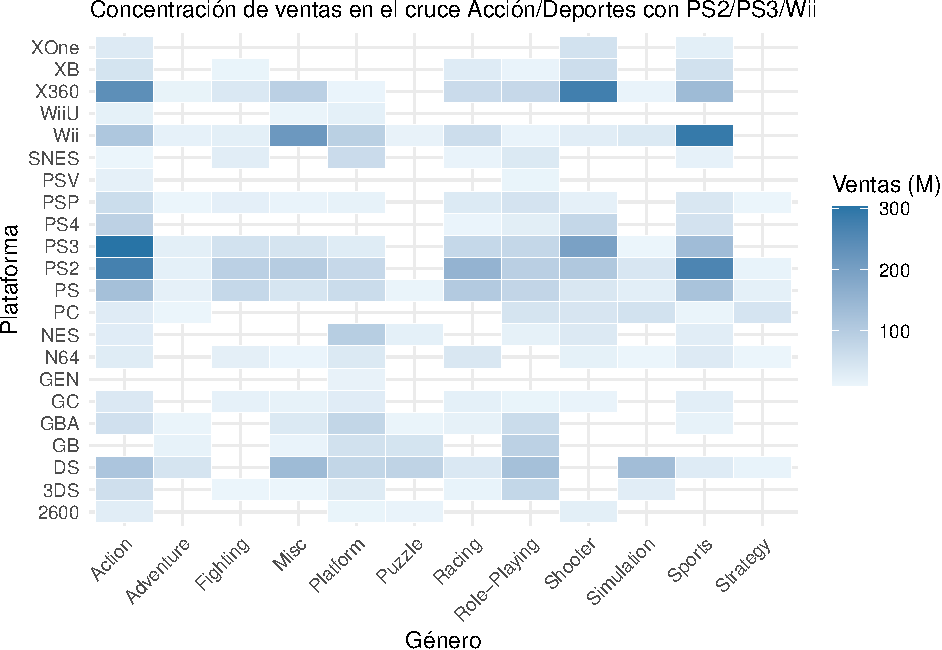
\includegraphics[width=0.9\linewidth,]{informe_files/figure-latex/unnamed-chunk-6-1} \end{center}

\chapter{Diagnóstico de Residuos del Modelo Lineal}

Como soporte al Marco Metodológico, se presentan los gráficos de
diagnóstico para validar los supuestos de un modelo de regresión lineal
simple (OLS) donde se intenta explicar las Ventas Globales en función de
las Ventas en Norteamérica.

\[ \text{Global\_Sales} = \beta_0 + \beta_1 (\text{NA\_Sales}) + \epsilon \]

\begin{center}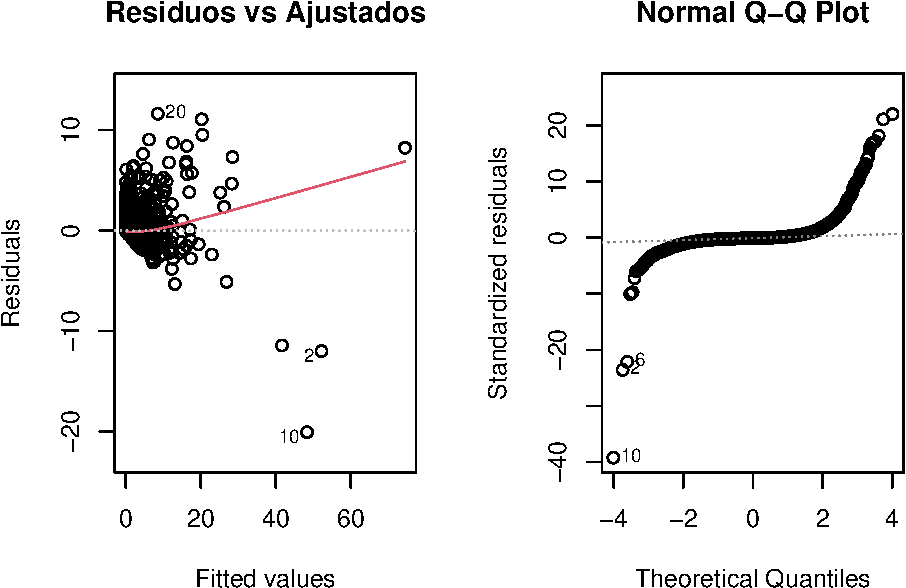
\includegraphics[width=0.9\linewidth,]{informe_files/figure-latex/unnamed-chunk-7-1} \end{center}

Como se observa en el gráfico Q-Q (derecha), los residuos se desvían
significativamente de la línea diagonal punteada en los cuantiles
superiores. Esto confirma que los errores no siguen una distribución
normal, validando la conclusión del Capítulo 3 sobre la necesidad de
usar modelos generalizados (GLM) o transformaciones logarítmicas para
proyecciones futuras.

%%%%%%%%%%%%%%%%%%%%%%%%%%%%%%%%%%%%%%%%%%%%%%%%%%%%%
%                   REFERENCIAS                     %
%%%%%%%%%%%%%%%%%%%%%%%%%%%%%%%%%%%%%%%%%%%%%%%%%%%%%
% Mantenemos la estructura natbib de tu plantilla
\renewcommand{\bibname}{Lista de Referencias}
\bibliographystyle{apalike} 
\bibliography{bibliografia.bib} 

%%%%%%%%%%%%%%%%%%%%%%%%%%%%%%%%%%%%%%%%%%%%%%%%%%%%%
%                   APÉNDICES                       %
%%%%%%%%%%%%%%%%%%%%%%%%%%%%%%%%%%%%%%%%%%%%%%%%%%%%%

\end{document}
